\section{ Filler lecture:Atmospheres }\label{sec:q4}    


\subsection*{a)}
First, Uranus and Neptune are located much further away from the sun, making their equilibrium temperature lower. This causes more condensation of methane, which changes the emissions spectrum. Especially higher-frequency molecule vibrations will be less common when the temperature is lower, reflected in the the much lower albedo values for the lower frequencies. Secondly, Uranus and Neptune have different mass and atmospheric compositions to Jupiter and Saturn, which can impact things like atmosphere transparency, which in turn impacts the measured albedo.

\subsection*{b)}
\begin{figure}[H]
    \centering
    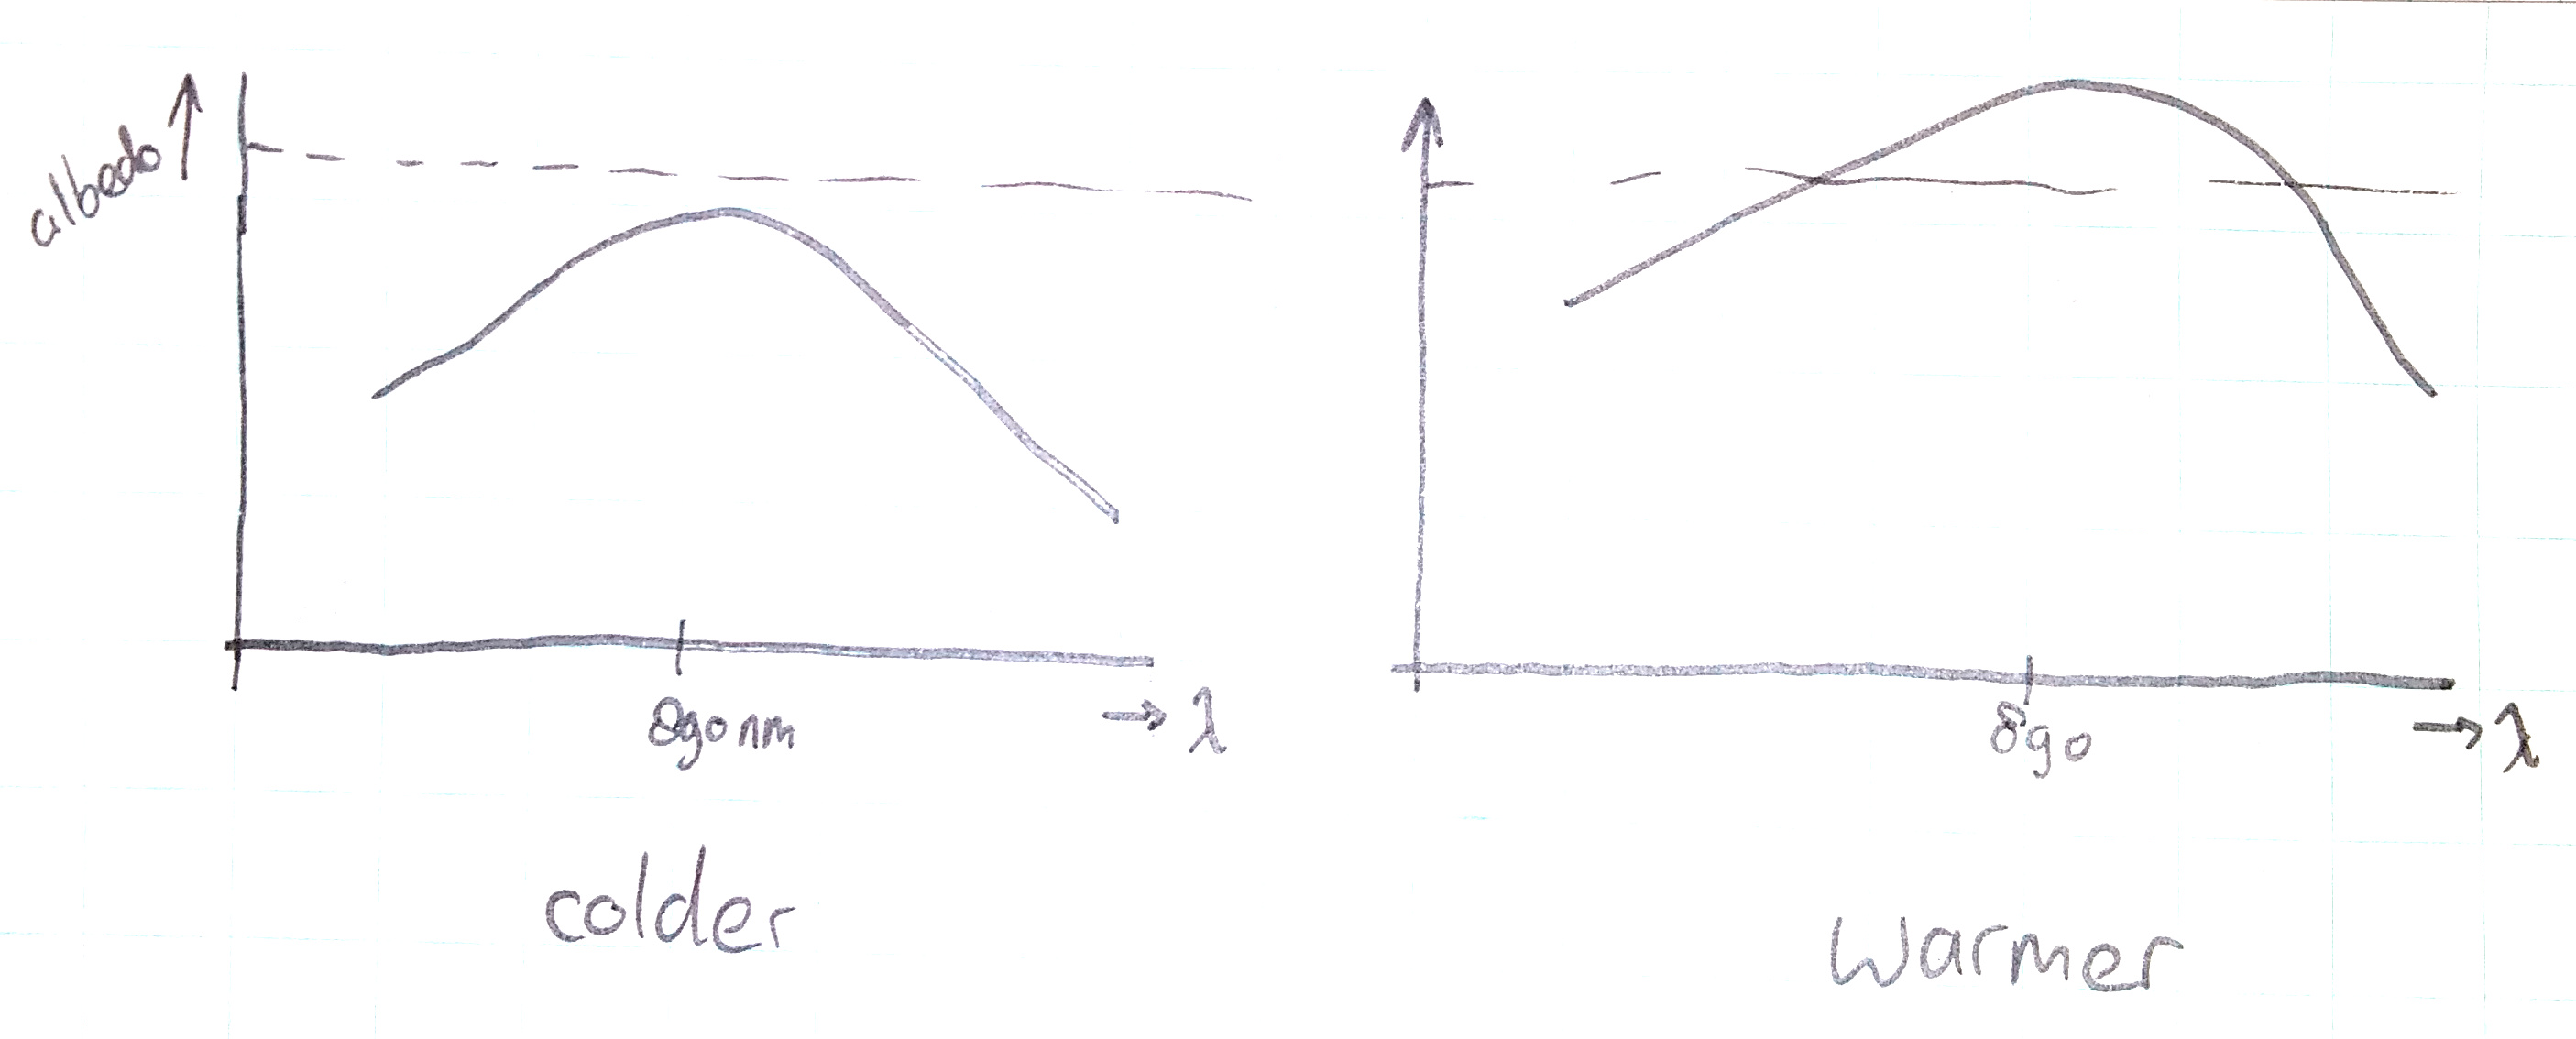
\includegraphics[width=0.8\textwidth]{figures/4b.jpg}
    %\caption{Caption}
    \label{fig:my_label4}
\end{figure}
The main take-away is that the albedo increases as the temperature increases, and the temperature is directly affected by the pressure. 

\subsection*{c)}
First, we make two assumptions:
\begin{enumerate}
    \item We assume that the two planets have the same bond albedo $A_B$.
    \item We assume that the two planets have the same emissivity $\epsilon$, since their atmospheric composition is similar.
\end{enumerate}

The equilibrium temperature is then purely dependant on the planet's distance to the sun. Since we already know the temperature of Uranus, we substitute the planet-specific data in the equation given in the question, and then divide the two:

\begin{equation}
    \begin{split}
        \dfrac{T_{Neptune}^4}{T_{Uranus}^4} = \dfrac{\frac{(1-A_B)}{4\epsilon \sigma} \frac{F_O}{r_{Neptune}^2}} {\frac{(1-A_B)}{4\epsilon \sigma} \frac{F_O}{r_{Uranus}^2}} \\
        \dfrac{T_{Neptune}^4}{T_{Uranus}^4} = \dfrac{r_{Uranus}^2}{r_{Neptune}^2}\\
        T_{Neptune}^4 = T_{Uranus} \sqrt[4]{\dfrac{r_{Uranus}^2}{r_{Neptune}^2}}\\
    \end{split}
\end{equation}

And so: 
\begin{equation}
    T_{Neptune}^4 = 60 \cdot \sqrt[4]{\dfrac{20^2}{40^2}} = 42.43 \; K\\
\end{equation}


\subsection*{d)}
\begin{itemize}
    \item Atmospheric composition can contribute to raising equilibrium temperature, especially if large amounts of greenhouse gases are present, such as $CO_2$ or $CH_4$. An extreme example of this is Venus, which is blanketed in a dense, heat-retaining atmosphere. 
    \item Internal heating, for example from lingering formation heat or radioactive decay of isotopes such as $^{40}$K or $^{232}$Th.
\end{itemize}

\subsection*{e)}
There are numerous effects, but an important one is the notion that Uranus' orbit is eccentric, causing it to move closer to and further from the sun. The formula presented in the question assumes a circular orbit of constant radius, and therefore the nuance of this effect is completely neglected.

\subsection*{f)}
